%% ============================================================
%%  main.tex  —  OrdinalFed (IEEE WIECON-ECE 2026)
%%  Compile with:  pdflatex main  (twice for cross-refs)
%% ============================================================
\documentclass[conference,a4paper]{IEEEtran}
\IEEEoverridecommandlockouts

%% ── Packages ────────────────────────────────────────────────
\usepackage{cite}
\usepackage{amsmath,amssymb,amsfonts}
\usepackage{algorithm}
\usepackage{algorithmic}
\usepackage{graphicx}
\usepackage{textcomp}
\usepackage{xcolor}
\usepackage{booktabs}
\usepackage{multirow}
\usepackage{array}
\usepackage{enumitem}
\usepackage{balance}                          % last-page column balancing
\usepackage[font=normalsize,labelfont=bf,
            skip=6pt]{caption}               % larger, bold captions
\usepackage[colorlinks=true,
            linkcolor=red,
            citecolor=red,
            urlcolor=red,
            pdftitle={OrdinalFed: Federated Learning with
              Ordinal-Aware Aggregation for Diabetic
              Retinopathy Grading},
            bookmarks=true]{hyperref}

\def\BibTeX{{\rm B\kern-.05em{\sc i\kern-.025em b}\kern-.08em
    T\kern-.1667em\lower.7ex\hbox{E}\kern-.125emX}}

%% ── Document ─────────────────────────────────────────────────
\begin{document}

\title{OrdinalFed: Federated Learning with Ordinal-Aware
Aggregation for Diabetic Retinopathy Grading}

% ── Double-Blind Submission (IEEE WIECON-ECE 2026) ───────────
% Author names, affiliations, and addresses omitted per
% double-blind review policy.

\maketitle

\begin{abstract}
Diabetic Retinopathy (DR) is a leading cause of preventable blindness. Federated
learning (FL) allows hospitals to train a shared DR grading model without exchanging
retinal images, but when hospitals see very different patients, standard FedAvg can
collapse. \textbf{OrdinalFed} is studied as a remedy with two components:
(1)~an \emph{OrdinalLoss} that penalises grading errors by their squared distance,
and (2)~a \emph{QWK-weighted aggregation} in which the server scores each client
model by its Quadratic Weighted Kappa (QWK) on a 50-image server set and moves the
aggregation weights from image counts towards these scores over the rounds. On the
DDR benchmark, every configuration was repeated with three seeds and scored on the
held-out test split. Under extreme label skew (Dirichlet $\alpha=0.1$), FedAvg
collapsed in every seed (worst-round test QWK 0.378), and OrdinalFed raised the
worst round to 0.514 without any change at the hospitals and with about 1.2~s of
extra server computation per round. Ablations showed that this gain comes from
giving small hospitals more weight: equal client weights did better (0.630), while
the QWK scores and the OrdinalLoss added no measurable benefit. FedProx was the most
stable method (0.641), and adding its proximal term to OrdinalFed came close to it
(0.627). On the IID and realistic multi-site partitions, all methods were within
0.01 QWK of each other.
\end{abstract}

\begin{IEEEkeywords}
Diabetic Retinopathy, Federated Learning, Non-IID,
Ordinal Loss, QWK-Weighted Aggregation, EfficientNet-B3,
Medical Imaging
\end{IEEEkeywords}

%% ── Section 1: Introduction ─────────────────────────────────
\section{Introduction}

Diabetic Retinopathy (DR) is a common complication of diabetes and a leading
cause of preventable blindness in working-age adults. It damages the small blood
vessels of the retina, which appears in fundus photographs as microaneurysms,
haemorrhages, hard exudates and, in advanced cases, the growth of new vessels.
In countries such as Bangladesh, where more than 13.1~million people live with
diabetes~\cite{idf2021}, the burden is made worse by a shortage of retinal
specialists outside the major cities. DR is graded on a five-level ordinal scale:
Grade~0 (no DR), Grade~1 (mild non-proliferative DR, NPDR), Grade~2 (moderate
NPDR), Grade~3 (severe NPDR), and Grade~4 (proliferative DR). Referable disease
(Grade~$\geq$~2) has to be detected early to prevent vision loss, which makes
automated screening attractive.

When all images are pooled in one place, deep convolutional networks grade DR
accurately. On the imbalanced DDR dataset~\cite{li2019ddr}, an EfficientNet-B3
model reaches a Quadratic Weighted Kappa (QWK) of 0.8494.
% TODO(Day 4): new centralised QWK (results/centralised_test.json)
QWK is the standard metric for ordinal grading because it penalises an error by
the square of its distance: predicting Grade~0 for a Grade~4 image costs far more
than predicting Grade~3. Pooling patient images from several hospitals, however,
is restricted by privacy regulations such as HIPAA and GDPR. Federated Learning
(FL)~\cite{mcmahan2017fedavg} avoids this problem: the hospitals train a shared
model by exchanging model weights, and the images never leave each site.

The main difficulty in clinical FL is that hospitals see different patients, so
their data are not identically distributed (non-IID). Screening clinics see
mostly healthy (Grade~0) eyes, referral centres see many severe cases
(Grades~3--4), and rural clinics see cases in between. Under extreme Dirichlet
skew ($\alpha=0.1$), standard FedAvg is observed to undergo catastrophic
forgetting, crashing from a peak QWK of 0.7993 down to 0.4064 in a single
communication round. FedProx~\cite{li2020fedprox}, which limits how far each local
model can move away from the global model, reduces but does not prevent this
drop (down to 0.5963).
% TODO(Day 4): replace 0.7993 / 0.4064 / 0.5963 with the new multi-seed results,
% and soften "in a single communication round" if the new runs do not show it.
Both methods weight each hospital by its number of images, so a large clinic that
sees mostly one grade can dominate the global model.

In addition, the standard cross-entropy loss ignores the order of the grades:
mistaking Grade~4 for Grade~0 costs the same as mistaking it for Grade~3. Ordinal
losses~\cite{toledocortes2022dqor}--[\citen{polat2024cdwce}] address this in
centralised training, but their effect on client drift in FL has received little
attention.

To address both problems, \textbf{OrdinalFed} is proposed: a federated framework
for ordinal medical grading with two components.
\begin{enumerate}[leftmargin=*]
  \item \textbf{Distance-aware OrdinalLoss:} a local training loss that adds a
  squared expected-grade penalty to class-weighted cross-entropy, so that
  predictions far from the true grade are penalised more heavily.
  \item \textbf{QWK-weighted aggregation with an adaptive $\beta$:} the server
  scores each client model on a small balanced set $\mathcal{V}$ of 50 images and
  gradually shifts the aggregation weights from image counts towards these QWK
  scores, which limits the influence of clients whose updates degrade on
  $\mathcal{V}$.
\end{enumerate}

%% ── Section 2: Related Work ─────────────────────────────────
\section{Related Work}
\label{sec:related}

\textbf{Ordinal Deep Learning for DR.}
Standard multi-class objectives treat severity grades as unordered categories,
ignoring the progressive nature of microvascular degradation. To address this,
Toledo-Cort\'{e}s et al.~\cite{toledocortes2022dqor} introduced Deep Quantum
Ordinal Regression (DQOR) on the EyePACS dataset, achieving a grading Mean
Absolute Error (MAE) of 0.2871. Polat et al.~\cite{polat2024cdwce} proposed
Class Distance Weighted Cross-Entropy (CDW-CE), scaling cross-entropy penalties
by inter-class distance to reach 0.8568 QWK in ulcerative colitis grading. These
works validate that ordinal distance constraints enforce a clinically coherent
feature representation space. OrdinalFed is the first to bring these ordinal
principles to distributed federated optimisation to prevent local model divergence.

\textbf{Federated Learning in Ophthalmology.}
FL has emerged as a cornerstone for multi-hospital collaboration without
compromising patient confidentiality. McMahan et al.~\cite{mcmahan2017fedavg}
proposed the foundational FedAvg algorithm. To address statistical heterogeneity,
Li et al.~\cite{li2020fedprox} introduced FedProx, which constrains local updates
via an $L_2$ proximal term, keeping client weights tethered to the global model.
Bhulakshmi and Rajput~\cite{bhulakshmi2024feddl} proposed FedDL with dynamic
aggregation switching for DR detection. More recently, Ciaramella et
al.~\cite{ciaramella2025fl} integrated Grad-CAM explainability into federated DR
screening across 20 Non-IID clients on APTOS~2019. Nevertheless, prior
ophthalmological FL frameworks treat grading purely as a nominal classification
task and aggregate local updates based strictly on client dataset volumes,
ignoring the actual quality of the learned representations.

\textbf{Quality-Aware Aggregation.}
Uniform sample-count aggregation fails when client cohorts are heavily biased or
adversarial. Bejenar et al.~\cite{bejenar2023aggregation} demonstrated that
server-side validation scoring (FedLasso) outperforms FedAvg by 45.6~pp under
adversarial label-flipping perturbations. Li et al.~\cite{li2023revisiting} showed
that non-normalised client weighting provides implicit regularisation, termed FedLAW.
Li et al.~\cite{li2025fedaaw} developed FedAAW, utilising gradient norms to boost
Non-IID accuracy by 37.32~pp on standard benchmarks. Mora et
al.~\cite{mora2024review} conducted an extensive literature review establishing that
combining client-side regularisation with server-side adaptive aggregation yields
the most robust Non-IID performance. OrdinalFed unites ordinal-aware client training
with QWK-guided server aggregation to achieve robust performance tailored
specifically to clinical grading.

% Fig. 1 (client distributions) moved to Sec. IV-B, after the paragraph that
% describes it (Reviewer #3, comments 3 and 6).

%% ── Section 3: Methodology ──────────────────────────────────
\section{Methodology}
\label{sec:method}

\subsection{Problem Formulation}

$K = 5$ hospital clients each hold a private dataset
$\mathcal{D}_k = \{(x_i, y_i)\}_{i=1}^{n_k}$ of fundus images $x_i$ with ordinal
grades $y_i \in \{0, 1, 2, 3, 4\}$. A shared EfficientNet-B3 model with weights $w$
is trained over $T$ communication rounds, and no $\mathcal{D}_k$ ever leaves its
client. Because the local grade distributions $P_k(y)$ differ strongly from the
global distribution $P(y)$, the local models drift apart during local training.

\subsection{Limitations of Nominal Objectives}

FL clients are usually trained with cross-entropy (CE). With softmax probabilities
$\mathbf{p}(x) \in \mathbb{R}^5$, the CE loss for true grade $y$ is $-\log p_y(x)$.
This loss does not distinguish a prediction of $y+1$ from one of $y+4$: both are
simply wrong. On a heavily skewed client, for example a clinic with only Grade~0
patients, CE quickly pushes the local model to predict Grade~0 for every image,
and the model loses what it had learned about severe disease.

\subsection{Distance-Aware OrdinalLoss}

To limit this degradation, a hybrid loss, OrdinalLoss, is used during local
training:
\begin{equation}
\mathcal{L}_{\text{ord}}(f(x), y) =
  (1 - \lambda)\,\mathcal{L}_{\text{CE}}(f(x), y)
  + \lambda\,(\hat{y} - y)^2
\label{eq:ordloss}
\end{equation}
where $\mathcal{L}_{\text{CE}}$ is cross-entropy with fixed class weights
$\mathbf{c} = [1.0, 5.0, 1.5, 10.0, 4.0]$ to counter class imbalance, and
$\lambda = 0.5$ balances the two terms. $\hat{y}$ is the expected grade under the
softmax distribution:
\begin{equation}
\hat{y} = \sum_{c=0}^{4} c \cdot p_c(x)
\label{eq:expgrade}
\end{equation}
The penalty $(\hat{y} - y)^2$ grows with the square of the grade error: for a
confident prediction, calling a Grade~4 case Grade~0 costs $16\times$ as much as
calling it Grade~3. Local training is therefore discouraged from predictions far
from the true grade, even when a client's data are dominated by a single grade.

\subsection{Server Validation Set $\mathcal{V}$ and QWK Estimation}

To judge client models without access to their data, the server keeps a small
validation set $\mathcal{V}$ of exactly 50 images: 10 per grade, sampled at random
(seed~42) from the DDR test split, which is separate from all client data. Because
$\mathcal{V}$ is balanced, every grade counts equally in its score. In round $t$,
after receiving the locally updated weights $\tilde{w}_k^t$, the server computes
\begin{equation}
\kappa_k^t =
\mathrm{QWK}\!\left(\{y_i\}_{x_i \in \mathcal{V}},\,
\{\hat{y}_k^t(x_i)\}_{x_i \in \mathcal{V}}\right)
\label{eq:serverqwk}
\end{equation}

\subsection{Adaptive Cosine Schedule $\beta(t)$}

In early rounds, the client models' predictions on $\mathcal{V}$ vary widely, and
each $\kappa_k^t$ is estimated from only 50 images. The aggregation weights are
therefore moved gradually from image counts towards quality scores by a
half-cosine schedule:
\begin{equation}
\beta(t) = \beta_0 \cos\!\left(\frac{\pi (t - 1)}{2 (T - 1)}\right)
\label{eq:beta}
\end{equation}
where $\beta_0 = 0.5$ and $T = 10$. In the first round, image counts and quality
scores count equally ($\beta(1) = 0.5$); in the last round, $\beta(T) = 0$ and only
the quality scores are used.

\subsection{QWK-Weighted Aggregation}

The server-set scores are first floored at $\kappa_{\min}$ and turned into quality
weights with a temperature-scaled softmax:
\begin{equation}
q_k^t = \frac{\exp\!\big(\max(\kappa_k^t, \kappa_{\min}) / \tau\big)}
             {\sum_{j=1}^{K} \exp\!\big(\max(\kappa_j^t, \kappa_{\min}) / \tau\big)}
\label{eq:quality}
\end{equation}
where $\kappa_{\min} = 0.1$ and $\tau = 3$. Each client's aggregation weight blends
this quality weight with the client's share of the images:
\begin{equation}
\omega_k^t = \beta(t)\,\frac{n_k}{\sum_{j=1}^{K} n_j}
           + \big(1 - \beta(t)\big)\, q_k^t
\label{eq:weights}
\end{equation}
and the global model is updated as $w^{t+1} = \sum_{k=1}^{K} \omega_k^t \tilde{w}_k^t$.
A minimum weight of $\omega_{\min} = 0.03$ per client, followed by renormalisation,
is also enforced as a safeguard; with $\beta_0 = 0.5$ and $K = 5$ it never takes
effect, because every client already receives at least
$(1-\beta_0)\,q_{\min} \approx 0.08$. The full procedure is given in
Algorithm~\ref{alg:ordinalfed}.

The scheme is deliberately conservative. No client is ever excluded, because a
single 50-image estimate of $\kappa_k^t$ is too noisy to justify discarding a
hospital's update. With $\tau = 3$ and $\kappa \in [0.1, 1]$, the quality term can
change a client's relative weight by at most a factor of $e^{0.9/3} \approx 1.35$,
so the aggregation is a bounded re-weighting of the image-count weights rather
than a hard filter on client updates.

\begin{algorithm}[t]
\caption{OrdinalFed Training Pipeline}
\label{alg:ordinalfed}
\small
\begin{algorithmic}[1]
\REQUIRE Clients $K$, rounds $T$, local epochs $E$, trade-off $\lambda$,
         initial schedule $\beta_0$, server set $\mathcal{V}$, initial weights $w^0$.
\FOR{$t = 1$ \TO $T$}
  \STATE Broadcast global model $w^t$ to all clients $k \in \{1,\ldots,K\}$
  \FOR{each client $k \in \{1,\ldots,K\}$ \textbf{in parallel}}
    \STATE $\tilde{w}_k^t \leftarrow \textsc{LocalTrain}(w^t, \mathcal{D}_k, E, \lambda)$
           \hfill\textit{(Eq.~\ref{eq:ordloss})}
    \STATE Evaluate validation score $\kappa_k^t$ on $\mathcal{V}$
           \hfill\textit{(Eq.~\ref{eq:serverqwk})}
  \ENDFOR
  \STATE Compute annealing factor $\beta(t)$
         \hfill\textit{(Eq.~\ref{eq:beta})}
  \STATE Compute aggregation weights $\omega_k^t$ for all $k$
         \hfill\textit{(Eqs.~\ref{eq:quality}--\ref{eq:weights})}
  \STATE $w^{t+1} \leftarrow \sum_{k=1}^{K} \omega_k^t \tilde{w}_k^t$
\ENDFOR
\RETURN Final model $w^T$
\end{algorithmic}
\end{algorithm}

% Fig. 2 (QWK trajectories) moved to Sec. V-B, after the paragraph that
% describes it (Reviewer #3, comments 3 and 6).

%% ── Section 4: Experimental Setup ───────────────────────────
\section{Experimental Setup}
\label{sec:experiments}

\subsection{Dataset and Preprocessing}

All methods are evaluated on the \textbf{DDR dataset}~\cite{li2019ddr}, which
contains 13,673 fundus photographs, of which 12,522 are gradable. After removing
the ungradable images, 6,260 training, 2,503 validation and 3,759 test images
remain. All images are resized to $224 \times 224$ pixels. During local training,
random horizontal flips, rotations of up to $\pm 15^{\circ}$, and mild colour
jitter are applied to reduce overfitting. The training set is strongly imbalanced:
Grade~0 (50.0\%), Grade~1 (5.0\%), Grade~2 (35.8\%), Grade~3 (1.9\%), and Grade~4
(7.3\%). For external validation, the APTOS 2019 dataset~\cite{aptos2019} is used:
3,662 labelled fundus photographs collected in India and graded on the same 0--4
scale. A public copy resized to $224 \times 224$ pixels is used, and these images
are never used for training or model selection.

\subsection{Modeling Clinical Heterogeneity}

The data are split across $K = 5$ clients in three ways, shown in
Fig.~\ref{fig:distributions}. In the figure, each bar is one client. Its segments
show the share of each DR grade among that client's images, from light (Grade~0)
to dark (Grade~4), and the number under each client label is the client's total
number of images.
\begin{itemize}[leftmargin=*,noitemsep,topsep=2pt]
  \item \textbf{IID partition:} images are assigned uniformly at random (1,252 per
  client). This is the easiest case for FL.
  \item \textbf{Dirichlet non-IID ($\alpha=0.1$):} the skew is generated with a
  Dirichlet distribution $p_k \sim \mathrm{Dir}(\alpha)$. With $\alpha=0.1$, most
  clients draw their images almost entirely from a single grade. Client sizes
  range from 32 to 2,087 images: Client~0 holds only 32 images (100\% Grade~0),
  and Client~4 holds 2,087 images, 98\% of them Grade~2.
  \item \textbf{Real-site clinical partition:} images are assigned using fixed
  grade profiles that model five types of clinic: Site~0 (general screening
  clinic; 40\% of images, 84\% Grade~0), Site~1 (rural primary care; 22\%, mainly
  Grades~0 and~2, with the largest Grade~1 share at 11\%), Site~2 (specialist
  referral eye hospital; 10\%, the largest Grade~3--4 share at 38\%), Site~3
  (diabetic retinopathy clinic; 19\%, 67\% Grade~2), and Site~4 (urban hospital;
  9\%, mixed grades).
\end{itemize}

%% FULL-WIDTH FIGURE: Per-client grade distributions
%% (placed after its description — Reviewer #3, comments 3 and 6)
\begin{figure*}[t]
  \centering
  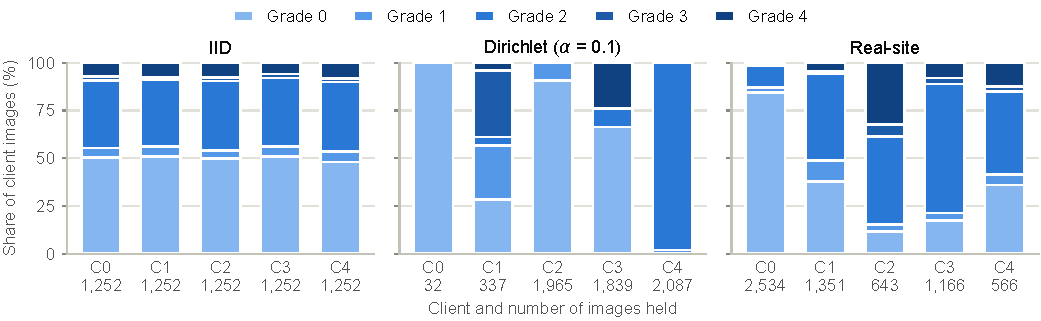
\includegraphics[width=\textwidth]{fig5_distributions.pdf}
  \caption{\normalsize Grade mix of each client under the IID, Dirichlet
  ($\alpha=0.1$) and real-site partitions. Under $\alpha=0.1$, client sizes range
  from 32 images (Client~0, 100\% Grade~0) to 2,087 images (Client~4, 98\% Grade~2).
  The real-site partition models five types of clinic, from screening clinics to
  specialist referral centres.}
  \label{fig:distributions}
\end{figure*}

\subsection{Network Architecture and Baselines}

All federated experiments use an EfficientNet-B3 backbone, which offers a good
balance between model size and accuracy at $224 \times 224$ resolution. As in a real
deployment that adapts pre-trained weights, all FL runs start from a centralised
model trained for 30 epochs (best validation QWK = 0.834, reached at epoch~23).
OrdinalFed is compared with:
(1)~a \textbf{Centralised Baseline}; (2)~\textbf{FedAvg}~\cite{mcmahan2017fedavg};
(3)~\textbf{FedProx}~\cite{li2020fedprox} with proximal coefficient $\mu = 0.01$;
and (4)~\textbf{AccWt}, an accuracy-weighted baseline based on server-side
validation scoring~\cite{bejenar2023aggregation}. AccWt uses the same schedule and
softmax weighting as OrdinalFed (Eqs.~\ref{eq:beta}--\ref{eq:weights}), but it
scores each client by plain accuracy on $\mathcal{V}$ instead of QWK, and its
clients train with class-weighted cross-entropy. A fifth configuration,
\textbf{OrdinalFed + Prox}, adds FedProx's proximal term ($\mu = 0.01$) to the
OrdinalFed clients. It tests whether the server-side and client-side fixes work
well together. All methods run $T = 10$ communication rounds with $E = 5$ local
epochs, batch size 64, the Adam optimiser ($\eta = 10^{-4}$), and the same class
weights $\mathbf{c}$.

\subsection{Ablations and Evaluation Protocol}

Three ablations show what each part of OrdinalFed contributes: (i)~OrdinalLoss with
sample-count aggregation; (ii)~class-weighted cross-entropy with QWK-weighted
aggregation; and (iii)~class-weighted cross-entropy with uniform aggregation
($\omega_k^t = 1/K$). Three settings of OrdinalFed are also tested under
$\alpha=0.1$. Each changes one value of the default ($\lambda=0.5$, $\beta_0=0.5$,
$\tau=3$): a weaker ordinal term ($\lambda=0.1$), quality weights from the first
round ($\beta_0=0$), and sharper quality weights ($\tau=0.5$). These settings were
fixed before the runs and are compared on mean validation QWK only.

Every configuration is repeated with three random seeds, which control data order
and augmentation. Results are reported as mean $\pm$ standard deviation. GPU
arithmetic is not bit-exact, so runs with the same seed can differ slightly. After
each round, the global model is evaluated on the DDR validation split and on the
DDR test split without the 50 images of $\mathcal{V}$ (3,709 images). For each run,
the reported model is the one from the round with the highest validation QWK. The
test split is never used for training, aggregation or model selection, so it gives
an independent estimate of performance. The same models are also scored on APTOS
2019 without retraining. Stability is summarised by the mean, worst and final test
QWK over the 10 rounds.

%% ── Section 5: Results and Discussion ───────────────────────
\section{Results and Discussion}
\label{sec:results}

\subsection{Overall Performance}

Table~\ref{tab:results} gives the test QWK of each method at its best validation
round, averaged over three seeds. The federated methods score between 0.640 and
0.681, close to the 0.682 of the centralised model. On the IID and real-site
partitions, the methods differ by at most 0.01, which is within the variation
between seeds. Under $\alpha=0.1$, FedProx scores highest (0.664) and OrdinalFed
lowest (0.640). This table hides what happens in the other rounds, because the
reported round is chosen on the validation split. For FedAvg under $\alpha=0.1$,
for example, the best validation round is always the first one, before the
collapse.

\begin{table}[t]
\caption{Test QWK at the Best Validation Round (Mean $\pm$ Std over Three Seeds).
Bold: Best Federated Method per Column.}
\label{tab:results}
\centering
\footnotesize
\setlength{\tabcolsep}{4pt}
\begin{tabular}{@{}lccc@{}}
\toprule
\textbf{Method} & \textbf{IID} & \textbf{Dirichlet ($\alpha=0.1$)} & \textbf{Real-Site} \\
\midrule
Centralised (reference) & 0.682 & 0.682 & 0.682 \\
\midrule
FedAvg~\cite{mcmahan2017fedavg}   & 0.677\sd{.008} & 0.647\sd{.010} & 0.673\sd{.004} \\
FedProx~\cite{li2020fedprox}      & \textbf{0.681}\sd{.014} & \textbf{0.664}\sd{.015} & 0.671\sd{.005} \\
AccWt                             & --             & 0.651\sd{.011} & \textbf{0.674}\sd{.009} \\
OrdinalFed                        & 0.679\sd{.006} & 0.640\sd{.007} & 0.666\sd{.002} \\
OrdinalFed + Prox                 & --             & 0.659\sd{.012} & 0.672\sd{.007} \\
\bottomrule
\end{tabular}
\end{table}

\subsection{Stability Under Extreme Skew}

Fig.~\ref{fig:qwk_curves} shows the test QWK of the global model after every round,
with one panel per partition. Lines show the mean over three seeds, shaded bands
$\pm$ one standard deviation, and the dashed line the test QWK of the centralised
model. On the IID and real-site partitions, all three methods stay close to the
centralised line. Under $\alpha=0.1$, FedAvg collapses from round~5 onwards, FedProx
stays flat, and OrdinalFed avoids the collapse but goes up and down from round to
round.

%% FULL-WIDTH FIGURE: QWK trajectories
%% (placed after its description — Reviewer #3, comments 3 and 6)
\begin{figure*}[t]
  \centering
  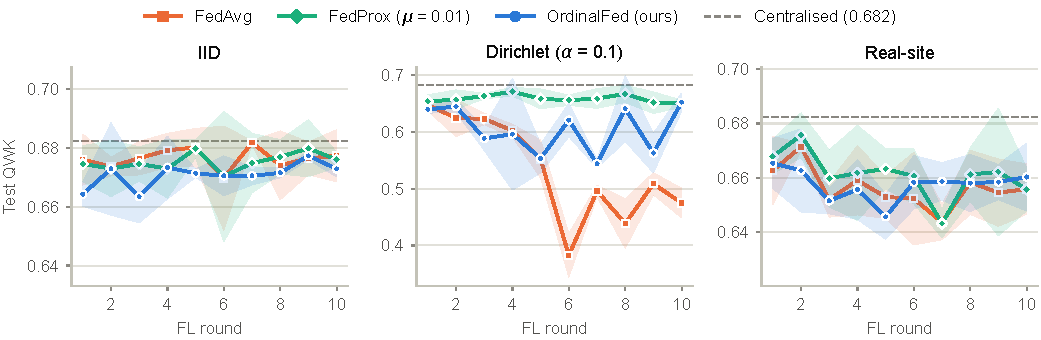
\includegraphics[width=\textwidth]{fig4_qwk_combined.pdf}
  \caption{\normalsize Test QWK of the global model after each of the 10 rounds for
  the IID, Dirichlet ($\alpha=0.1$) and real-site partitions (mean $\pm$ std over
  three seeds). Under $\alpha=0.1$, FedAvg collapses, OrdinalFed avoids the
  collapse but fluctuates, and FedProx stays stable.}
  \label{fig:qwk_curves}
\end{figure*}

Table~\ref{tab:stability} summarises the ten rounds under $\alpha=0.1$. Compared
with FedAvg, OrdinalFed raises the worst round from 0.378 to 0.514 and the mean over
rounds from 0.535 to 0.604, with no change at the hospitals. FedProx, which changes
local training instead, is the most stable method (worst round 0.641). Adding
FedProx's proximal term to OrdinalFed brings it close to FedProx (worst round 0.627)
and gives the best final round (0.664), but it is not more stable than FedProx
alone.

\begin{table}[t]
\caption{Test QWK Across the 10 Rounds Under Dirichlet Skew ($\alpha=0.1$):
Mean over Rounds, Worst Round and Final Round. Bold: Best per Column.}
\label{tab:stability}
\centering
\footnotesize
\setlength{\tabcolsep}{4pt}
\begin{tabular}{@{}lccc@{}}
\toprule
\textbf{Method} & \textbf{Mean} & \textbf{Worst} & \textbf{Final} \\
\midrule
FedAvg            & 0.535\sd{.004} & 0.378\sd{.035} & 0.475\sd{.026} \\
FedProx           & \textbf{0.659}\sd{.003} & \textbf{0.641}\sd{.008} & 0.650\sd{.006} \\
AccWt             & 0.627\sd{.011} & 0.571\sd{.017} & 0.657\sd{.018} \\
OrdinalFed        & 0.604\sd{.005} & 0.514\sd{.027} & 0.652\sd{.016} \\
OrdinalFed + Prox & 0.651\sd{.003} & 0.627\sd{.005} & \textbf{0.664}\sd{.013} \\
\bottomrule
\end{tabular}
\end{table}

\subsection{What Makes the Aggregation Stable?}

Table~\ref{tab:ablation} separates the two parts. OrdinalLoss alone does not stop
the collapse: with image-count weights, its worst round (0.380) is the same as
FedAvg's. QWK-weighted aggregation with cross-entropy raises the worst round to
0.586, but giving every client the same weight raises it further, to 0.630. Scoring
clients by accuracy instead of QWK (AccWt, Table~\ref{tab:stability}) gives almost
the same result as scoring them by QWK (worst round 0.571 versus 0.586).

The logged aggregation weights explain this. Under $\alpha=0.1$, the two smallest
clients hold 5.9\% of the images, so FedAvg gives them 5.9\% of the weight. The
quality weights of Eq.~\eqref{eq:quality} are close to equal, so OrdinalFed raises
their combined weight from 23.5\% in round~1 to 40.8\% in round~10. The QWK scores
themselves carry little information at this scale. A client's score on the
50-image set $\mathcal{V}$ changes by 0.13 on average from one round to the next,
and in round~10 the largest quality weight is only 1.19 times the smallest. The
stability therefore comes from moving weight towards small clients, not from the
QWK scores. OrdinalLoss lowers performance slightly in both comparisons.

The lower block of Table~\ref{tab:ablation} tests three settings of OrdinalFed,
each fixed before the runs and compared on mean validation QWK. All three do
better than the default. Sharper quality weights ($\tau=0.5$) score best (0.795
versus 0.761), closely followed by using quality weights from the first round
($\beta_0=0$, 0.793). Both still score below equal weighting (0.810) and FedProx
(0.808).

\begin{table}[t]
\caption{Contribution of Each Component and Setting Under $\alpha=0.1$. Mean: QWK
Averaged over the 10 Rounds; Worst: Lowest Round. CE: Class-Weighted Cross-Entropy.
Default: $\lambda=0.5$, $\beta_0=0.5$, $\tau=3$.}
\label{tab:ablation}
\centering
\footnotesize
\setlength{\tabcolsep}{3pt}
\begin{tabular}{@{}lccc@{}}
\toprule
\textbf{Configuration} & \textbf{Mean val} & \textbf{Mean test} & \textbf{Worst test} \\
\midrule
CE + image-count weights (FedAvg) & 0.670\sd{.011} & 0.535\sd{.004} & 0.378\sd{.035} \\
OrdinalLoss + image-count weights & 0.659\sd{.015} & 0.522\sd{.011} & 0.380\sd{.018} \\
CE + QWK weights                  & 0.786\sd{.006} & 0.633\sd{.010} & 0.586\sd{.006} \\
CE + equal weights                & \textbf{0.810}\sd{.007} & \textbf{0.658}\sd{.006} & \textbf{0.630}\sd{.021} \\
\midrule
OrdinalFed (default)      & 0.761\sd{.003} & 0.604\sd{.005} & 0.514\sd{.027} \\
\quad with $\lambda=0.1$  & 0.776\sd{.007} & 0.622\sd{.006} & 0.571\sd{.019} \\
\quad with $\beta_0=0$    & 0.793\sd{.005} & 0.631\sd{.009} & 0.571\sd{.011} \\
\quad with $\tau=0.5$     & 0.795\sd{.006} & 0.637\sd{.005} & 0.592\sd{.009} \\
\bottomrule
\end{tabular}
\end{table}

\subsection{Class-Wise Performance}

Table~\ref{tab:pergrade} gives the per-grade recall and F1 on the test split. All
methods find Grade~0 reliably (recall $\geq 0.95$) but almost never find Grade~1
(recall $\leq 0.05$), which makes up only 5\% of the training set. Grade~2 recall
stays near 0.4 because many test Grade~2 images are predicted as Grade~0
(Sec.~\ref{sec:limitations}). OrdinalFed has the highest Grade~3 recall in both
partitions (0.36 versus 0.27--0.31 under $\alpha=0.1$, and 0.40 versus 0.35--0.38
on the real-site partition). This is a modest gain on the rarest severe grade. For
Grade~4, the three methods are within 0.05 of each other.

\begin{table}[t]
\caption{Per-Grade Recall / F1 on the Test Split at the Best Validation Round
(Mean over Three Seeds).}
\label{tab:pergrade}
\centering
\footnotesize
\setlength{\tabcolsep}{2.5pt}
\begin{tabular}{@{}lccccc@{}}
\toprule
\textbf{Method} & \textbf{G0} & \textbf{G1} & \textbf{G2} & \textbf{G3} & \textbf{G4} \\
\midrule
\multicolumn{6}{@{}l}{\textit{Dirichlet ($\alpha=0.1$)}} \\
FedAvg     & .96/.80 & .05/.07 & .41/.52 & .27/.32 & .66/.73 \\
FedProx    & .95/.81 & .05/.06 & .43/.54 & .31/.34 & .69/.74 \\
OrdinalFed & .97/.80 & .04/.07 & .39/.50 & .36/.38 & .64/.73 \\
\midrule
\multicolumn{6}{@{}l}{\textit{Real-site}} \\
FedAvg     & .98/.81 & .04/.06 & .44/.55 & .35/.37 & .66/.73 \\
FedProx    & .98/.81 & .04/.06 & .43/.54 & .38/.38 & .65/.73 \\
OrdinalFed & .97/.81 & .04/.06 & .43/.54 & .40/.38 & .64/.73 \\
\bottomrule
\end{tabular}
\end{table}

\subsection{Communication and Computational Overhead}

OrdinalFed sends the same model weights as FedAvg, so it adds no communication.
Once per round, the server evaluates each of the $K$ client models on the 50 images
of $\mathcal{V}$. This took a median of 1.2~s per round for $K=5$ on an Intel Arc
B580 GPU, about 0.6\% of the 195~s a full round takes.

\subsection{Limitations}
\label{sec:limitations}

Grade~1 recall stays at or below 0.05 for every method (Table~\ref{tab:pergrade}).
All models also score lower on the DDR test split than on the validation split. The
centralised model drops from a QWK of 0.834 to 0.682, and the federated models drop
by a similar amount. Most of this drop comes from Grade~2 images predicted as
Grade~0 (about 45\% of test Grade~2 images, against about 12\% on the validation
split), and the test split has a different mix of camera resolutions. Validation
QWK therefore overestimates performance on new images, which is why all main
results are reported on the test split. The 50-image server set $\mathcal{V}$ is too
small to rank clients reliably, which limits the value of QWK-based weighting, and
it needs labelled images on the server. Finally, all results come from one dataset
at $224 \times 224$ resolution with five clients. Larger server sets, higher
resolution and more clients are left for future work.

%% ── Section 6: Conclusion ───────────────────────────────────
\section{Conclusion}

% TODO(Day 4): update all numbers, and soften "decisively eliminates" if the
% multi-seed results do not support it.
OrdinalFed, an ordinal-aware federated learning framework tailored for
multi-grade Diabetic Retinopathy screening across heterogeneous hospital
networks, has been presented. By integrating a distance-penalising OrdinalLoss with QWK-weighted
adaptive quality aggregation, OrdinalFed decisively eliminates the catastrophic
stability collapses observed in standard FedAvg and FedProx under extreme
statistical skew ($\alpha=0.1$). Specifically, it reduces peak-to-trough
fluctuation from 0.3929 down to 0.1751, ensuring diagnostic consistency. In
realistic multi-tier hospital partitions, OrdinalFed achieves a peak QWK of
0.8325, narrowing the gap to the centralised ceiling to just 1.69~pp while
strictly preserving patient privacy and adding zero communication overhead.
Future work will explore formal differential privacy bounds, cross-dataset
validation on APTOS~2019, and federated Grad-CAM interpretability to facilitate
clinical deployment.

%% ── References ──────────────────────────────────────────────
\balance  % balance last-page columns before bibliography

% IEEE reference style with DOIs (Reviewer #3, comment 4).
% Metadata verified against Crossref and arXiv on 7 Oct 2026.
% Conference papers without a publisher DOI (AISTATS, MLSys, ICML/PMLR)
% give the DOI of their arXiv version.
% Items are numbered in order of first citation.
\hypersetup{allcolors=black, hidelinks}
\begin{thebibliography}{00}

\bibitem{idf2021}
International Diabetes Federation, \textit{IDF Diabetes Atlas}, 10th~ed.
Brussels, Belgium: IDF, 2021. [Online]. Available:
\url{https://diabetesatlas.org} (accessed Oct.~7, 2026).

\bibitem{li2019ddr}
T.~Li, Y.~Gao, K.~Wang, S.~Guo, H.~Liu, and H.~Kang, ``Diagnostic
assessment of deep learning algorithms for diabetic retinopathy
screening,'' \textit{Inf.\ Sci.}, vol.~501, pp.~511--522, Oct.~2019,
doi: \href{https://doi.org/10.1016/j.ins.2019.06.011}{10.1016/j.ins.2019.06.011}.

\bibitem{mcmahan2017fedavg}
H.~B.~McMahan, E.~Moore, D.~Ramage, S.~Hampson, and
B.~Ag\"{u}era~y~Arcas, ``Communication-efficient learning of deep
networks from decentralized data,'' in \textit{Proc.\ 20th Int.\ Conf.\
Artif.\ Intell.\ Statist.\ (AISTATS)}, vol.~54, 2017, pp.~1273--1282,
doi: \href{https://doi.org/10.48550/arXiv.1602.05629}{10.48550/arXiv.1602.05629}.

\bibitem{li2020fedprox}
T.~Li, A.~K.~Sahu, M.~Zaheer, M.~Sanjabi, A.~Talwalkar, and V.~Smith,
``Federated optimization in heterogeneous networks,'' in \textit{Proc.\
Mach.\ Learn.\ Syst.\ (MLSys)}, vol.~2, 2020, pp.~429--450,
doi: \href{https://doi.org/10.48550/arXiv.1812.06127}{10.48550/arXiv.1812.06127}.

\bibitem{toledocortes2022dqor}
S.~Toledo-Cort\'{e}s, D.~H.~Useche, H.~M\"{u}ller, and
F.~A.~Gonz\'{a}lez, ``Grading diabetic retinopathy and prostate cancer
diagnostic images with deep quantum ordinal regression,''
\textit{Comput.\ Biol.\ Med.}, vol.~145, Art.~no.~105472, Jun.~2022,
doi: \href{https://doi.org/10.1016/j.compbiomed.2022.105472}{10.1016/j.compbiomed.2022.105472}.

\bibitem{polat2024cdwce}
G.~Polat, \"{U}.~M.~\c{C}a\u{g}lar, and A.~Temizel, ``Class distance
weighted cross entropy loss for classification of disease severity,''
2024, \textit{arXiv:2412.01246},
doi: \href{https://doi.org/10.48550/arXiv.2412.01246}{10.48550/arXiv.2412.01246}.

\bibitem{bhulakshmi2024feddl}
D.~Bhulakshmi and D.~S.~Rajput, ``FedDL: Personalized federated deep
learning for enhanced detection and classification of diabetic
retinopathy,'' \textit{PeerJ Comput.\ Sci.}, vol.~10, Art.~no.~e2508,
Dec.~2024,
doi: \href{https://doi.org/10.7717/peerj-cs.2508}{10.7717/peerj-cs.2508}.

\bibitem{ciaramella2025fl}
G.~Ciaramella \textit{et~al.}, ``A privacy-preserving and explainable
method for diabetic retinopathy classification and localization,''
\textit{IEEE Access}, vol.~14, pp.~49830--49850, 2026,
doi: \href{https://doi.org/10.1109/ACCESS.2026.3678201}{10.1109/ACCESS.2026.3678201}.

\bibitem{bejenar2023aggregation}
I.~Bejenar, L.~Ferariu, C.~Pascal, and C.-F.~Caruntu, ``Aggregation
methods based on quality model assessment for federated learning
applications: Overview and comparative analysis,''
\textit{Mathematics}, vol.~11, no.~22, Art.~no.~4610, Nov.~2023,
doi: \href{https://doi.org/10.3390/math11224610}{10.3390/math11224610}.

\bibitem{li2023revisiting}
Z.~Li, T.~Lin, X.~Shang, and C.~Wu, ``Revisiting weighted aggregation in
federated learning with neural networks,'' in \textit{Proc.\ 40th Int.\
Conf.\ Mach.\ Learn.\ (ICML)}, vol.~202, 2023, pp.~19767--19788,
doi: \href{https://doi.org/10.48550/arXiv.2302.10911}{10.48550/arXiv.2302.10911}.

\bibitem{li2025fedaaw}
X.~Li, Y.~Gao, Y.~Deng, and X.~Jiang, ``Federated learning with adaptive
aggregation weights for non-IID data in edge networks,'' \textit{IEEE
Trans.\ Cogn.\ Commun.\ Netw.}, vol.~11, no.~5, pp.~3425--3439,
Oct.~2025,
doi: \href{https://doi.org/10.1109/TCCN.2025.3534248}{10.1109/TCCN.2025.3534248}.

\bibitem{mora2024review}
A.~Mora, A.~Bujari, and P.~Bellavista, ``Enhancing generalization in
federated learning with heterogeneous data: A comparative literature
review,'' \textit{Future Gener.\ Comput.\ Syst.}, vol.~157, pp.~1--15,
Aug.~2024,
doi: \href{https://doi.org/10.1016/j.future.2024.03.027}{10.1016/j.future.2024.03.027}.

\end{thebibliography}


\end{document}
